\chapter{Regulación de la presión arterial y ejercicio}\label{ch:b2:blood-pressure}

Si uno se levanta de golpe tras estar tumbado, durante un segundo medio
litro de \omterm{def:b2:blood-circulation:blood}{sangre} se desplaza a las \omterm{def:b2:blood-circulation:vessels}{venas} de las piernas; el \omterm{def:b2:heart:anatomy}{corazón}, que
recibe menos, bombea menos, la presión en la cabeza cae, y el encéfalo
--- que está a \qty{40}{cm} por encima del \omterm{def:b2:heart:anatomy}{corazón} y no puede almacenar
oxígeno --- está a uno o dos segundos del desmayo. Casi nunca llega a
producirse, porque en un solo latido un reflejo ha contraído las
\omterm{def:b2:blood-circulation:vessels}{arteriolas} y acelerado el \omterm{def:b2:heart:anatomy}{corazón}. Si se corre para alcanzar un autobús,
los músculos necesitan diez veces la \omterm{def:b2:blood-circulation:blood}{sangre} que tenían en reposo; la
obtienen en un minuto, y la presión que la impulsa se mantiene estable
mientras la resistencia de todo el cuerpo cae en dos tercios. Este
capítulo trata de esa regulación: qué fija la presión, cómo se percibe,
el reflejo rápido y las hormonas lentas que la corrigen, y cómo el sistema
se reorganiza, en lugar de quedar anulado, durante el ejercicio.

\section{Qué es la presión}

\begin{theorem}[La ecuación de la circulación]\label{thm:b2:blood-pressure:equation}
\index{presión arterial media}\index{resistencia periférica total}
La \omterm{thm:b2:blood-pressure:equation}{presión arterial media} $\bar P$ es el producto de lo que introduce el
\omterm{def:b2:heart:anatomy}{corazón} y de lo que dejan salir los vasos:
\[
\bar P - P_{\text{ven}} = Q\,R, \qquad Q = f\times V_s,
\]
donde $Q$ es el \omterm{thm:b2:heart:starling}{gasto cardíaco} (la frecuencia cardíaca $f$ por el \omterm{prop:b2:heart:cycle}{volumen
sistólico} $V_s$), $R$ la \omterm{thm:b2:blood-pressure:equation}{resistencia periférica total} --- las \omterm{def:b2:blood-circulation:vessels}{arteriolas} de
todos los órganos en paralelo --- y $P_{\text{ven}}$ la presión venosa,
cercana a cero. En reposo, $\qty{5}{L/min}\times\qty{1.08}{mmHg.s/mL}$ da
\qty{90}{mmHg}. Toda regulación de la presión actúa sobre una de tres
magnitudes: la frecuencia, el \omterm{prop:b2:heart:cycle}{volumen sistólico} (a través del llenado y de
la contractilidad del \cref{ch:b2:heart}) o la resistencia (a través del
radio arteriolar, elevado a la cuarta potencia). Como los órganos están en
paralelo, el flujo hacia cada uno es su parte de la presión dividida por su
propia resistencia: dilatar las \omterm{def:b2:blood-circulation:vessels}{arteriolas} de un órgano aumenta su flujo
sin cambiar el de los demás, siempre que se mantenga la presión --- y
mantener la presión es precisamente para lo que sirve la regulación.
\end{theorem}
\begin{proof}
La ley de Ohm para un fluido: el flujo a través de una resistencia es la
caída de presión a través de ella dividida por la resistencia (Poiseuille,
\cref{ch:b2:blood-circulation}); para resistencias en paralelo los flujos se
suman y $1/R = \sum 1/R_i$. La presión media a lo largo de un latido es
aproximadamente la diastólica más un tercio de la \omterm{thm:b2:blood-circulation:windkessel}{presión del pulso}:
$80 + 40/3 = \qty{93}{mmHg}$.
\end{proof}

\begin{omfigure}
\begin{tikzpicture}[every node/.style={font=\scriptsize}, >=stealth]
  \node[draw, rounded corners, fill=omThm!15, minimum width=2.4cm, minimum height=1cm, align=center] (heart) at (0,0) {corazón\\$Q = f\,V_s$};
  \draw[very thick, omThm] (1.2,0) -- (2.4,0);
  \draw[very thick, omThm] (2.4,-2.4) -- (2.4,2.4);
  \foreach \y/\org/\r in {2.0/{encéfalo}/{$R_1$}, 1.0/{músculo cardíaco}/{$R_2$}, 0/{intestino e hígado}/{$R_3$}, -1.0/{riñones}/{$R_4$}, -2.0/{músculo, piel}/{$R_5$}} {
    \draw[very thick, omThm] (2.4,\y) -- (3.6,\y);
    \draw[thick, decorate, decoration={zigzag, segment length=4pt, amplitude=2pt}] (3.6,\y) -- (5.0,\y);
    \node[above] at (4.3,\y+0.05) {\org};
    \node[below] at (4.3,\y-0.05) {\r};
    \draw[very thick, omDef] (5.0,\y) -- (6.2,\y);
  }
  \draw[very thick, omDef] (6.2,-2.4) -- (6.2,2.4);
  \draw[very thick, omDef] (6.2,0) -- (7.4,0) |- (0,-3.2) -- (0,-0.5);
  \node[omThm, above] at (1.8,0.05) {$\bar P$};
  \node[omDef, below] at (3.7,-3.2) {venas, $P_{\text{ven}} \approx 0$};
  \node[anchor=west, align=left] at (7.8,1.5) {órganos en paralelo:\\$1/R = \sum 1/R_i$\\flujo al órgano $i$: $\bar P/R_i$};
\end{tikzpicture}

{\small La circulación como circuito: una bomba, una presión y las
resistencias arteriolares de los órganos en paralelo. Cada órgano toma
$\bar P/R_i$; la regulación mantiene $\bar P$ mientras las $R_i$ se
ajustan a la demanda.}
\end{omfigure}

\begin{proposition}[Por qué debe regularse la presión]\label{prop:b2:blood-pressure:why}
Si es demasiado baja, el encéfalo --- a \qty{40}{cm} por encima del \omterm{def:b2:heart:anatomy}{corazón} en
un adulto de pie, lo que cuesta \qty{31}{mmHg} de columna hidrostática ---
y el propio músculo cardíaco quedan mal irrigados: el encéfalo falla en
segundos. Si es demasiado alta, los vasos se dañan: la pared arterial se
engrosa y se endurece, los glomérulos del riñón se cicatrizan, la retina
sangra y el \omterm{def:b2:heart:anatomy}{corazón} se esfuerza contra la presión hasta que falla. La
presión también debe mantenerse estable mientras las demandas de los
órganos cambian en un orden de magnitud --- el intestino tras una comida,
los músculos durante el ejercicio, la piel con el calor --- y mientras el
propio volumen sanguíneo se pierde por una hemorragia o por el sudor. Dos
sistemas se encargan de ello: un reflejo nervioso que actúa en un solo
latido sobre la frecuencia, el \omterm{prop:b2:heart:cycle}{volumen sistólico} y la resistencia, y unos
sistemas hormonales que actúan a lo largo de horas y días sobre la
resistencia y, sobre todo, sobre el volumen sanguíneo a través del riñón.
\end{proposition}

\begin{omfigure}
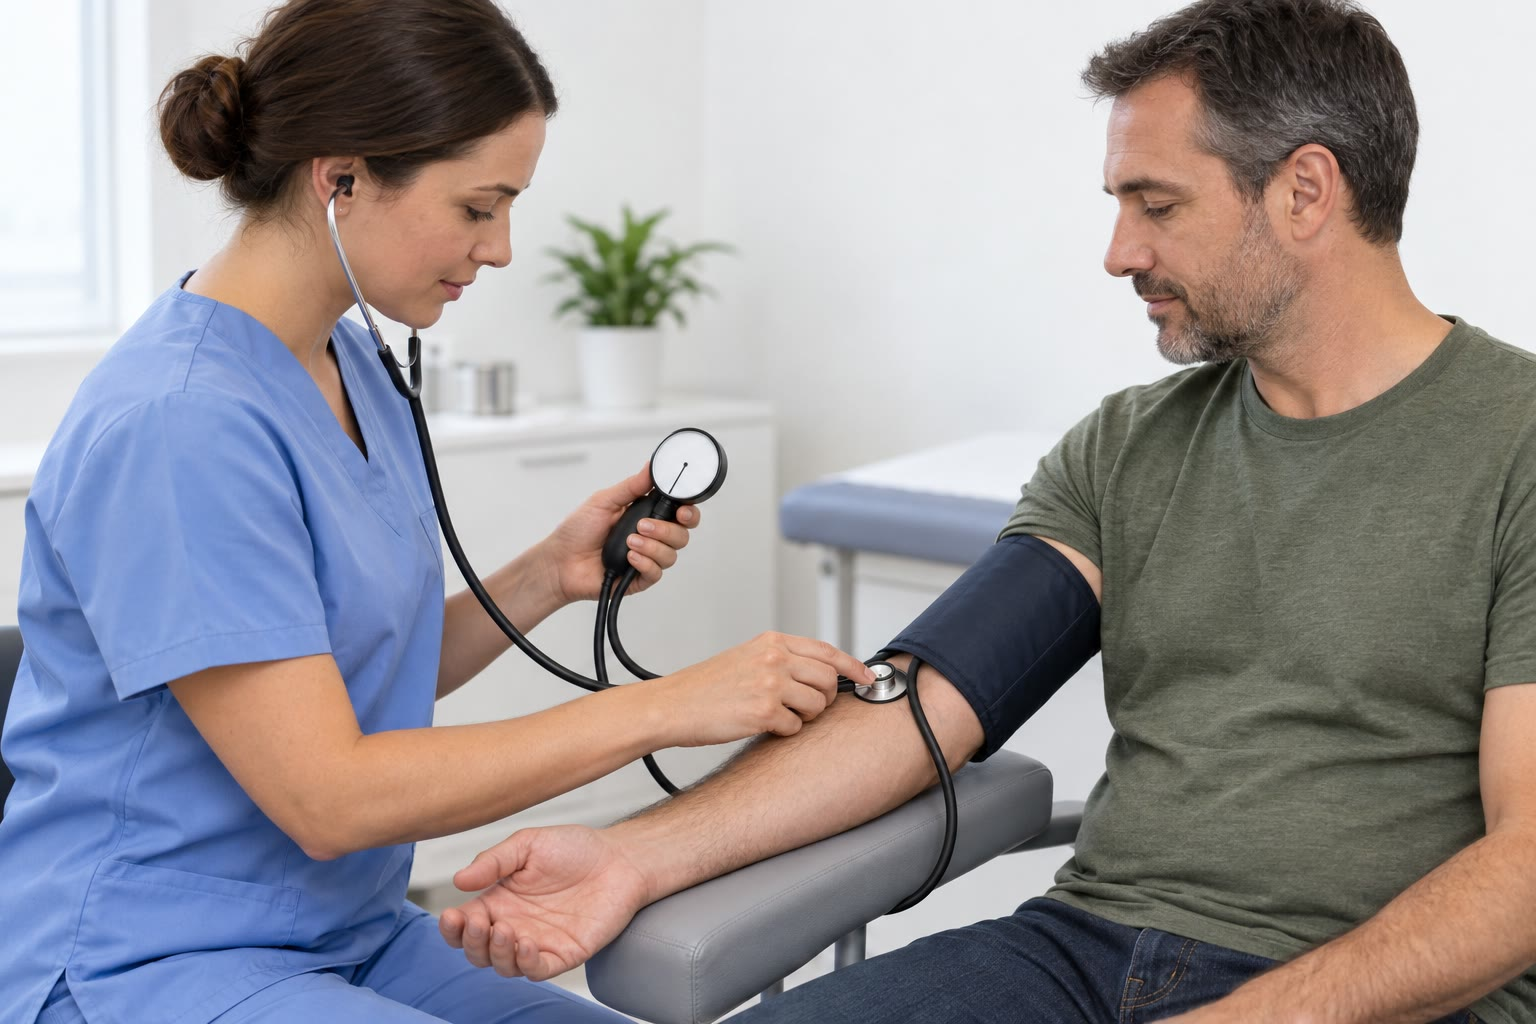
\includegraphics[width=0.6\linewidth]{images/book4/ai/b4-18-blood-pressure-cuff.jpg}

{\small La medida de la presión. El manguito se infla por encima de la
presión sistólica, de modo que no pasa \omterm{def:b2:blood-circulation:blood}{sangre}; al desinflarlo, los
primeros ruidos del flujo turbulento bajo el estetoscopio marcan la
presión sistólica, y su desaparición, cuando la \omterm{def:b2:blood-circulation:vessels}{arteria} permanece abierta
durante todo el ciclo, marca la diastólica.}
\end{omfigure}

\section{El bucle rápido: el barorreflejo}

\begin{definition}[El barorreflejo]\label{def:b2:blood-pressure:baroreflex}
\index{barorreceptor}\index{barorreflejo}\index{centro vasomotor}\index{sistema nervioso autónomo}
Unos receptores de estiramiento de las paredes de los senos carotídeos (en
la bifurcación de cada \omterm{def:b2:blood-circulation:vessels}{arteria} carótida, bajo la mandíbula) y del cayado
aórtico --- los \emph{barorreceptores} --- descargan con una frecuencia que
aumenta con la presión que los distiende, y más deprisa si la presión
sube. Sus nervios llegan a los \emph{centros cardiovasculares} del bulbo
raquídeo, que controlan las dos ramas de la eferencia autónoma: el vago,
cuya acetilcolina ralentiza el \omterm{prop:b2:heart:conduction}{nódulo sinoauricular}, y los nervios
simpáticos, cuya noradrenalina acelera el nódulo, refuerza el \omterm{def:b2:heart:anatomy}{ventrículo},
contrae las \omterm{def:b2:blood-circulation:vessels}{arteriolas} (lo que eleva $R$) y contrae las \omterm{def:b2:blood-circulation:vessels}{venas} (lo que
empuja la \omterm{def:b2:blood-circulation:blood}{sangre} almacenada hacia el \omterm{def:b2:heart:anatomy}{corazón} y aumenta el llenado). Una
subida de la presión aumenta la descarga de los barorreceptores, lo que
excita el vago e inhibe la eferencia simpática: la frecuencia cae, las
\omterm{def:b2:blood-circulation:vessels}{arteriolas} se relajan y la presión baja. Una bajada produce lo contrario.
El bucle es una \emph{retroalimentación negativa} con un valor de consigna
cercano a \qty{95}{mmHg}, un retraso de alrededor de un segundo y una
ganancia tal que una perturbación queda corregida hasta la quinta parte de
su tamaño: es la razón de que uno no se desmaye al ponerse de pie.
\end{definition}
\begin{proof}[Evidencia]
Hering (1923) observó que presionar el seno carotídeo ralentizaba el
\omterm{def:b2:heart:anatomy}{corazón} y bajaba la presión, y que seccionar el nervio del seno suprimía la
respuesta. Perfundir un seno carotídeo aislado a presiones fijadas
mientras se registraba la presión arterial del animal dio la curva
sigmoide del reflejo: la presión del animal baja a medida que se eleva la
presión del seno, de forma pronunciada en torno a \qty{100}{mmHg} y poco
fuera de \qtyrange{60}{160}{mmHg}. Los perros con los nervios del seno y
aórticos seccionados mantienen durante días una presión media normal,
pero extremadamente variable de un minuto a otro --- el reflejo es un
amortiguador, no el que fija el nivel a largo plazo.
\end{proof}

\begin{omfigure}
\begin{tikzpicture}[every node/.style={font=\scriptsize}, >=stealth]
  \node[draw, rounded corners, fill=omDef!15, align=center] (bp) at (0,0) {presión arterial\\$\bar P$};
  \node[draw, rounded corners, fill=omDef!15, align=center] (baro) at (4.2,0) {barorreceptores\\seno carotídeo, cayado aórtico\\descarga $\uparrow$ con $\bar P$};
  \node[draw, rounded corners, fill=omProp!20, align=center] (med) at (8.6,0) {bulbo raquídeo:\\centros cardiovasculares};
  \node[draw, rounded corners, fill=omThm!15, align=center] (vag) at (8.6,-2.2) {vago $\uparrow$: frecuencia $\downarrow$};
  \node[draw, rounded corners, fill=omThm!15, align=center] (sym) at (4.2,-2.2) {simpático $\downarrow$: frecuencia, contractilidad,\\tono arteriolar y venoso $\downarrow$};
  \draw[->, thick] (bp) -- (baro); \draw[->, thick] (baro) -- (med);
  \draw[->, thick] (med) -- (vag); \draw[->, thick] (med) -- (sym);
  \draw[->, thick] (sym.west) -| (bp.south) node[pos=0.75, left, align=right] {$Q\downarrow$, $R\downarrow$:\\$\bar P\downarrow$};
  \draw[->, thick] (vag.west) -- (sym.east);
  \node[anchor=north, align=center] at (4.3,-3.2) {a una subida de la presión responde una bajada: retroalimentación negativa, retraso de un segundo};
\end{tikzpicture}

{\small El \omterm{def:b2:blood-pressure:baroreflex}{barorreflejo}. Una subida de la presión arterial aumenta la
descarga de los \omterm{def:b2:blood-pressure:baroreflex}{barorreceptores}, lo que lleva al bulbo raquídeo a
ralentizar el \omterm{def:b2:heart:anatomy}{corazón} y relajar los vasos; una bajada produce lo contrario.}
\end{omfigure}

\begin{theorem}[La ganancia de un bucle de retroalimentación negativa]\label{thm:b2:blood-pressure:gain}
\index{ganancia de la retroalimentación}
Si una perturbación, sin regulación, cambiara la presión en $\Delta P_0$, y
el bucle respondiera a toda desviación $\Delta P$ con una corrección de
$-G\,\Delta P$ (la \emph{ganancia en bucle abierto} $G$), la desviación que
queda una vez que el bucle ha actuado es
\[
\Delta P = \frac{\Delta P_0}{1 + G}.
\]
El \omterm{def:b2:blood-pressure:baroreflex}{barorreflejo} tiene $G \approx 4$: ponerse de pie, que haría caer la
presión en el \omterm{def:b2:heart:anatomy}{corazón} unos \qty{40}{mmHg}, la hace caer
\qty{8}{mmHg}; una hemorragia que reduciría la presión a la mitad la baja
una décima parte --- hasta que la pérdida supera lo que pueden disimular
unos vasos más contraídos y un \omterm{def:b2:heart:anatomy}{corazón} más rápido. El reflejo no suprime
una perturbación; la divide por cinco. Y se \emph{reajusta}: mantenidos
durante horas a una nueva presión, los \omterm{def:b2:blood-pressure:baroreflex}{barorreceptores} se adaptan y
defienden el nuevo nivel, y por eso el reflejo no puede curar la
hipertensión y el nivel a largo plazo se fija en otro lugar.
\end{theorem}
\begin{proof}
La desviación final es la perturbación más la corrección:
$\Delta P = \Delta P_0 - G\,\Delta P$, de donde $\Delta P(1 + G) =
\Delta P_0$. Con $G = 4$, $\Delta P = \Delta P_0/5$.
\end{proof}

\begin{omfigure}
\begin{tikzpicture}
\begin{axis}[
  width=0.7\linewidth, height=5.4cm,
  axis x line=bottom, axis y line=left,
  xmin=40, xmax=180, ymin=40, ymax=160,
  xlabel={presión en el seno carotídeo (\unit{mmHg})}, ylabel={presión arterial resultante (\unit{mmHg})},
  xlabel style={font=\small, at={(axis description cs:0.5,-0.13)}, anchor=north},
  ylabel style={font=\small},
  tick label style={font=\small}, xtick={60,100,140}, ytick={60,100,140},
  clip=false,
]
\addplot[very thick, omDef, domain=40:180, samples=80] {100 + 50*tanh((100-x)/25)};
\addplot[thick, dashed, gray, domain=40:180, samples=2] {x};
\fill[omDef] (axis cs:100,100) circle (2pt); \draw[gray] (axis cs:101,100) -- (axis cs:124,110); \node[font=\scriptsize, anchor=west] at (axis cs:125,110) {consigna};
\node[font=\scriptsize, anchor=west, align=left] at (axis cs:46,112) {pendiente $-G$\\cerca de la consigna};
\end{axis}
\end{tikzpicture}

{\small La curva del \omterm{def:b2:blood-pressure:baroreflex}{barorreflejo}: la presión en la que se estabiliza el
cuerpo cuando el seno aislado se mantiene a una presión dada. Su pendiente
en el valor de consigna es la ganancia; fuera de
\qtyrange{60}{160}{mmHg} el reflejo está saturado.}
\end{omfigure}

\section{Los bucles lentos: las hormonas y el riñón}

\begin{proposition}[Renina, angiotensina, aldosterona y el volumen]\label{prop:b2:blood-pressure:raas}
\index{sistema renina--angiotensina}\index{aldosterona}\index{hormona antidiurética}\index{péptido natriurético}
A lo largo de horas y días, la presión la fija el \emph{volumen
sanguíneo}, y el volumen, el riñón. Cuando la presión o el sodio que llega
al riñón disminuyen, o cuando los nervios simpáticos descargan, unas
células de las \omterm{def:b2:blood-circulation:vessels}{arteriolas} del riñón liberan a la \omterm{def:b2:blood-circulation:blood}{sangre} la enzima
\emph{renina}; la renina corta una proteína plasmática y da la
\emph{angiotensina I}, que una enzima de los \omterm{def:b2:blood-circulation:vessels}{capilares} pulmonares
convierte en \emph{angiotensina II} --- el vasoconstrictor más potente del
cuerpo, que eleva $R$ en minutos, y una hormona que hace que la corteza
suprarrenal secrete \emph{aldosterona}, que hace que el riñón retenga
sodio, y con él agua, durante los días siguientes. La \emph{\omterm{prop:b2:blood-pressure:raas}{hormona
antidiurética}} de la hipófisis (vasopresina), liberada cuando la \omterm{def:b2:blood-circulation:blood}{sangre} se
concentra o su volumen disminuye, hace que el riñón retenga agua
directamente y también contrae los vasos. Y cuando las \omterm{def:b2:heart:anatomy}{aurículas} se
distienden en exceso por un volumen demasiado grande, secretan el
\emph{\omterm{prop:b2:blood-pressure:raas}{péptido natriurético}}, que hace que el riñón excrete sodio y agua.
El riñón es así el árbitro final: puede excretar o retener litros, y una
presión que se mantiene por encima del valor de consigna del riñón se
corrige, a lo largo de días, mediante la pérdida de volumen --- salvo que
el propio valor de consigna del riñón esté elevado, que es lo que ocurre en
la mayoría de las hipertensiones. (La maquinaria propia del riñón es el
tema del volumen del tercer año.)
\end{proposition}
\begin{proof}[Evidencia]
Goldblatt (1934) estrechó la \omterm{def:b2:blood-circulation:vessels}{arteria} de uno de los riñones de un perro:
el animal se volvió hipertenso en pocos días y siguió siéndolo; se
descubrió que el riñón mal irrigado liberaba renina, y extirparlo curaba
al animal. Los fármacos que bloquean la conversión de la angiotensina
(inhibidores de la ECA) o su receptor bajan la presión de la mayoría de
los hipertensos, y un riñón trasplantado de una cepa de ratas hipertensas
vuelve hipertenso a un receptor normal.
\end{proof}

\begin{omfigure}
\begin{tikzpicture}[every node/.style={font=\scriptsize}, >=stealth]
  \node[draw, rounded corners, fill=omDef!15, align=center] (fall) at (0,0) {la presión o el volumen disminuyen;\\los nervios simpáticos descargan};
  \node[draw, rounded corners, fill=omProp!20, align=center] (renin) at (4.4,0) {el riñón libera\\renina};
  \node[draw, rounded corners, fill=omProp!20, align=center] (ang) at (8.6,0) {angiotensina II\\(formada en la sangre y el pulmón)};
  \node[draw, rounded corners, fill=omThm!15, align=center] (vc) at (8.6,-2.0) {vasoconstricción:\\$R\uparrow$ en minutos};
  \node[draw, rounded corners, fill=omThm!15, align=center] (ald) at (4.4,-2.0) {aldosterona (suprarrenal):\\Na$^+$ y agua retenidos\\durante días --- volumen $\uparrow$};
  \draw[->, thick] (fall) -- (renin); \draw[->, thick] (renin) -- (ang);
  \draw[->, thick] (ang) -- (vc); \draw[->, thick] (ang) -- (ald);
  \draw[->, thick] (ald.west) -| (fall.south) node[pos=0.85, left, align=right] {presión\\restablecida};
  \draw[->, thick] (vc.west) -- (ald.east);
  \node[draw, rounded corners, fill=omExo!25, align=center] (anp) at (0,-2.0) {aurículas distendidas:\\péptido natriurético,\\sal y agua excretadas};
  \draw[->, thick, dashed] (anp.north) -- (fall.south);
\end{tikzpicture}

{\small El bucle lento. Una bajada de la presión pone en marcha la renina,
la angiotensina II y la aldosterona: constricción en minutos y retención de
sal y agua a lo largo de días. A un volumen excesivo responde el \omterm{prop:b2:blood-pressure:raas}{péptido
natriurético} de las \omterm{def:b2:heart:anatomy}{aurículas}.}
\end{omfigure}

\begin{example}[Una hemorragia]\label{ex:b2:blood-pressure:haemorrhage}
Un donante da \qty{500}{mL}, una décima parte de la \omterm{def:b2:blood-circulation:blood}{sangre}. En segundos, el
\omterm{def:b2:blood-pressure:baroreflex}{barorreflejo} contrae las \omterm{def:b2:blood-circulation:vessels}{arteriolas} y las \omterm{def:b2:blood-circulation:vessels}{venas} y acelera el \omterm{def:b2:heart:anatomy}{corazón}: la
presión apenas se mueve, la piel se vuelve pálida y fría (sus \omterm{def:b2:blood-circulation:vessels}{arteriolas}
se han cerrado) y el pulso es más rápido. En minutos, la menor presión
\omterm{def:b2:blood-circulation:vessels}{capilar} permite que el líquido intersticial pase a los vasos (el
equilibrio de Starling del \cref{ch:b2:blood-circulation}), lo que
restablece la mitad del volumen hacia la hora siguiente; la renina, la
angiotensina y la \omterm{prop:b2:blood-pressure:raas}{hormona antidiurética} reducen la orina a un hilo, y
aparece la sed; a lo largo de días el riñón retiene sal y agua y el volumen
plasmático se recupera, y a lo largo de semanas la médula ósea repone los
\omterm{def:b2:blood-circulation:blood}{glóbulos rojos}. Una pérdida de \qty{2}{L} supera todo esto: el reflejo se
satura, la presión se desploma, los tejidos mal irrigados liberan lactato
y los \omterm{def:b2:blood-circulation:vessels}{capilares} pierden líquido --- el shock, del que solo la transfusión
saca al paciente.
\end{example}

\section{El ejercicio: el sistema reorganizado}

\begin{proposition}[El ejercicio]\label{prop:b2:blood-pressure:exercise}
\index{fisiología del ejercicio}\index{flujo sanguíneo muscular}\index{gasto cardíaco!ejercicio}
En un ejercicio intenso, el consumo de oxígeno de los músculos
esqueléticos se multiplica por veinte, y su flujo sanguíneo pasa de
\qty{1}{L/min} a \qty{20}{L/min}. Ocurren tres cosas a la vez. Localmente,
los metabolitos del músculo en actividad --- $\mathrm{CO_2}$, lactato,
adenosina, potasio, calor, oxígeno bajo --- relajan sus \omterm{def:b2:blood-circulation:vessels}{arteriolas}
(\emph{vasodilatación metabólica}) y abren los \omterm{def:b2:blood-circulation:vessels}{capilares}, lo que reduce la
resistencia del músculo a la décima parte. Centralmente, una orden de la
corteza motora al bulbo raquídeo, reforzada por señales de los propios
receptores de los músculos, reajusta el \omterm{def:b2:blood-pressure:baroreflex}{barorreflejo} a un valor de consigna
más alto e impulsa la eferencia simpática: frecuencia a 180, mayor
contractilidad, constricción de las \omterm{def:b2:blood-circulation:vessels}{arteriolas} del intestino, los riñones
y los músculos en reposo, y compresión de las \omterm{def:b2:blood-circulation:vessels}{venas}; la bomba muscular y
la respiración profunda devuelven la \omterm{def:b2:blood-circulation:blood}{sangre} más deprisa. El resultado es un
gasto de \qty{25}{L/min} con una resistencia total que es un tercio de la de
reposo, una presión sistólica de \qty{150}{mmHg} y una diastólica no más
alta que en reposo; cuatro quintas partes del flujo van al músculo, la
parte del encéfalo no cambia en términos absolutos, la del intestino se
reduce a la mitad y la de la piel aumenta para disipar el calor. El reflejo
no queda anulado, sino reajustado: defiende una presión más alta mientras
los vasos abren el cuerpo.
\end{proposition}

\begin{omfigure}
\begin{tikzpicture}
\begin{axis}[
  ybar, bar width=9pt,
  width=0.9\linewidth, height=6cm,
  ymin=0, ymax=22, ytick={0,5,10,15,20},
  ylabel={flujo sanguíneo (\unit{L/min})}, ylabel style={font=\small},
  symbolic x coords={brain, heart, gut and liver, kidneys, muscle, skin, other},
  xtick=data, xticklabels={encéfalo, corazón, intestino e hígado, riñones, músculo, piel, otros}, x tick label style={font=\scriptsize, rotate=30, anchor=north east},
  tick label style={font=\small},
  legend style={font=\scriptsize, at={(0.03,0.97)}, anchor=north west, draw=none},
  enlarge x limits=0.12,
  clip=false,
]
\addplot[fill=omDef!50, draw=omDef] coordinates {(brain,0.75) (heart,0.25) (gut and liver,1.4) (kidneys,1.1) (muscle,1.0) (skin,0.3) (other,0.2)};
\addlegendentry{reposo, \qty{5}{L/min}}
\addplot[fill=omThm!50, draw=omThm] coordinates {(brain,0.75) (heart,1.0) (gut and liver,0.6) (kidneys,0.6) (muscle,20) (skin,1.6) (other,0.45)};
\addlegendentry{ejercicio intenso, \qty{25}{L/min}}
\end{axis}
\end{tikzpicture}

{\small Adónde va la \omterm{def:b2:blood-circulation:blood}{sangre}. En un ejercicio intenso el gasto se multiplica
por cinco y se redistribuye: veinte veces más a los músculos, más al
\omterm{def:b2:heart:anatomy}{corazón} y a la piel, menos al intestino y a los riñones, lo mismo al
encéfalo.}
\end{omfigure}

\begin{theorem}[El aporte de oxígeno y el principio de Fick]\label{thm:b2:blood-pressure:fick}
\index{principio de Fick}\index{VO2max@$\dot V_{\mathrm{O_2}\max}$}
El oxígeno que consume un cuerpo por minuto es igual al \omterm{thm:b2:heart:starling}{gasto cardíaco}
por la diferencia de contenido de oxígeno entre la \omterm{def:b2:blood-circulation:blood}{sangre} arterial y la
\omterm{def:b2:blood-circulation:blood}{sangre} venosa mezclada:
\[
\dot V_{\mathrm{O_2}} = Q\,(C_a - C_v).
\]
En reposo, $\qty{5}{L/min}\times(200 - 150)\,\unit{mL/L} = \qty{250}{mL/min}$;
en el ejercicio máximo, $\qty{25}{L/min}\times(200 - 40) =
\qty{4000}{mL/min}$, un aumento de dieciséis veces a partir de un flujo
cinco veces mayor y una extracción tres veces mayor. Este ritmo máximo,
$\dot V_{\mathrm{O_2}\max}$, es la medida de referencia de la resistencia
aeróbica, y su techo es el \omterm{def:b2:heart:anatomy}{corazón}: los músculos podrían extraer todavía
más y los pulmones cargar todavía más, pero el gasto no puede subir más.
El entrenamiento aumenta el \omterm{prop:b2:heart:cycle}{volumen sistólico} (un \omterm{def:b2:heart:anatomy}{ventrículo} más grande y
más distensible, más volumen sanguíneo) y, con él, el gasto --- la
frecuencia en reposo de 45 del deportista es la señal de un \omterm{prop:b2:heart:cycle}{volumen
sistólico} de \qty{110}{mL} ---, y añade \omterm{def:b2:blood-circulation:vessels}{capilares} y mitocondrias al músculo
para que extraiga más. A la inversa, el \omterm{thm:b2:blood-pressure:fick}{principio de Fick} es la manera de
medir el propio gasto en un paciente, a partir del oxígeno consumido y de
las dos muestras de \omterm{def:b2:blood-circulation:blood}{sangre}.
\end{theorem}
\begin{proof}
Cada litro de \omterm{def:b2:blood-circulation:blood}{sangre} que atraviesa los tejidos deja en ellos $C_a - C_v$
mililitros de oxígeno, y pasan $Q$ litros por minuto; en estado
estacionario, eso es lo que captan los pulmones y consume el cuerpo.
Despejando $Q$ se obtiene la medida.
\end{proof}

\begin{example}[Ponerse de pie, desmayarse, y el astronauta]\label{ex:b2:blood-pressure:standing}
Al ponerse de pie, \qty{500}{mL} de \omterm{def:b2:blood-circulation:blood}{sangre} pasan a las \omterm{def:b2:blood-circulation:vessels}{venas} de las
piernas, el retorno venoso y el \omterm{prop:b2:heart:cycle}{volumen sistólico} caen un tercio, y la
presión en el seno carotídeo baja --- el \omterm{def:b2:blood-pressure:baroreflex}{barorreflejo} responde en un latido
con un \omterm{def:b2:heart:anatomy}{corazón} más rápido y unos vasos más contraídos, y la presión en la
cabeza se recupera en diez segundos. Un soldado inmóvil en un patio de
armas caluroso pierde la bomba muscular, acumula \omterm{def:b2:blood-circulation:blood}{sangre} en las \omterm{def:b2:blood-circulation:vessels}{venas}
dilatadas de la piel y se desmaya: tumbarlo lo cura de inmediato. Un
astronauta tras meses sin gravedad ha perdido un litro de volumen
sanguíneo (el riñón excretó lo que interpretó como un exceso cuando la
\omterm{def:b2:blood-circulation:blood}{sangre} se acumuló en el tórax), y al aterrizar el reflejo, desentrenado,
no consigue mantenerlo erguido. Y la jirafa, cuya cabeza está dos metros
por encima del \omterm{def:b2:heart:anatomy}{corazón}, funciona con una presión media de \qty{200}{mmHg}
y lleva medias de compresión hechas de piel --- la hidrostática del
\cref{ch:b2:blood-circulation} fija las exigencias, y los reflejos de este
capítulo las satisfacen.
\end{example}

\section{Ejercicios}

\begin{exercise}[$\star$]\label{exo:b2:blood-pressure:1}
Escríbase la ecuación que relaciona la presión media, el \omterm{thm:b2:heart:starling}{gasto cardíaco} y
la resistencia periférica, y enumérense las tres magnitudes que el cuerpo
puede cambiar y el órgano o tejido que cambia cada una.
\end{exercise}

\begin{exercise}[$\star$]\label{exo:b2:blood-pressure:2}
Descríbase el \omterm{def:b2:blood-pressure:baroreflex}{barorreflejo}: sensores, centro, efectores, signo de la
retroalimentación y retraso. ¿Qué le ocurre de un minuto a otro a la
presión de un animal cuyos nervios \omterm{def:b2:blood-pressure:baroreflex}{barorreceptores} han sido seccionados?
\end{exercise}

\begin{exercise}[$\star$]\label{exo:b2:blood-pressure:3}
Dese la secuencia renina $\to$ angiotensina $\to$ aldosterona, con el
órgano que fabrica cada una y lo que hace cada una, y dígase qué la pone
en marcha.
\end{exercise}

\begin{exercise}[$\star$]\label{exo:b2:blood-pressure:4}
Nómbrense los tres mecanismos que multiplican por veinte el flujo
sanguíneo de un músculo en actividad, y dígase qué órganos ceden flujo para
hacerlo posible.
\end{exercise}

\begin{exercise}[$\star\star$]\label{exo:b2:blood-pressure:5}
Calcúlese la presión media para $Q = \qty{5}{L/min}$ y $R =
\qty{1.2}{mmHg.s/mL}$; para $Q = \qty{20}{L/min}$ y $R =
\qty{0.35}{mmHg.s/mL}$. En el segundo caso, ¿en qué factor ha cambiado el
radio arteriolar medio?
\end{exercise}

\begin{exercise}[$\star\star$]\label{exo:b2:blood-pressure:6}
Una perturbación haría caer la presión \qty{30}{mmHg}. Calcúlese la caída
residual para ganancias del reflejo de 2, 4 y 8. Un fármaco reduce a la
mitad la ganancia del \omterm{def:b2:blood-pressure:baroreflex}{barorreflejo} de una paciente: ¿qué nota al ponerse
de pie?
\end{exercise}

\begin{exercise}[$\star\star$]\label{exo:b2:blood-pressure:7}
Densidad de la \omterm{def:b2:blood-circulation:blood}{sangre}, \qty{1060}{kg/m^3}; el encéfalo está \qty{40}{cm}
por encima del \omterm{def:b2:heart:anatomy}{corazón} en un adulto de pie, y los pies \qty{120}{cm} por
debajo. Calcúlense las diferencias de presión hidrostática en mmHg, y la
presión arterial en el encéfalo y en el tobillo cuando la del \omterm{def:b2:heart:anatomy}{corazón} es
de \qty{95}{mmHg}. ¿Qué necesita una jirafa con la cabeza \qty{2.5}{m} por
encima del \omterm{def:b2:heart:anatomy}{corazón}?
\end{exercise}

\begin{exercise}[$\star\star$]\label{exo:b2:blood-pressure:8}
Con el \omterm{thm:b2:blood-pressure:fick}{principio de Fick}, calcúlese el \omterm{thm:b2:heart:starling}{gasto cardíaco} de un paciente que
consume \qty{280}{mL} de oxígeno por minuto con un contenido arterial de
\qty{190}{mL/L} y un venoso mezclado de \qty{130}{mL/L}. Una deportista
consume \qty{5}{L/min} en su máximo con contenidos de 200 y
\qty{30}{mL/L}: calcúlense su gasto y, a una frecuencia de 190, su \omterm{prop:b2:heart:cycle}{volumen
sistólico}.
\end{exercise}

\begin{exercise}[$\star\star$]\label{exo:b2:blood-pressure:9}
Una hemorragia de \qty{800}{mL} bajaría, sin regulación, la presión en
\qty{35}{mmHg}. Dese la presión tras el \omterm{def:b2:blood-pressure:baroreflex}{barorreflejo} ($G = 4$), enumérense
las cuatro cosas que restablecen el volumen con sus escalas de tiempo, y
explíquese la piel pálida y fría.
\end{exercise}

\begin{exercise}[$\star\star\star$]\label{exo:b2:blood-pressure:10}
El músculo en reposo tiene $R = \qty{5}{mmHg.s/mL}$ y recibe
\qty{1}{L/min}; durante el ejercicio su resistencia cae a la décima parte.
Si la presión se mantuviera en \qty{95}{mmHg} y no cambiara nada más, ¿qué
flujo tomaría el músculo, y qué gasto necesitaría el \omterm{def:b2:heart:anatomy}{corazón}? Si, en
cambio, el gasto del \omterm{def:b2:heart:anatomy}{corazón} se mantuviera en \qty{5}{L/min}, ¿hasta dónde
caería la presión? Explíquese por qué el cuerpo no hace ninguna de las dos
cosas y qué hace.
\end{exercise}

\begin{exercise}[$\star\star\star$]\label{exo:b2:blood-pressure:11}
Goldblatt estrechó una \omterm{def:b2:blood-circulation:vessels}{arteria} renal; el perro se volvió hipertenso de
forma permanente, con respuestas barorreflejas normales. Explíquese (a) por
qué el riñón elevó la presión, (b) por qué el \omterm{def:b2:blood-pressure:baroreflex}{barorreflejo} no lo impidió,
(c) por qué extirpar el riñón lo curó, (d) qué habría hecho un inhibidor de
la ECA.
\end{exercise}

\begin{exercise}[$\star\star\star$]\label{exo:b2:blood-pressure:12}
``El \omterm{def:b2:blood-pressure:baroreflex}{barorreflejo} es un amortiguador; el riñón es un termostato.''
Discútanse las escalas de tiempo, las ganancias y los valores de consigna
de los dos sistemas, y lo que cada uno puede y no puede hacer ante una
presión elevada de forma crónica.
\end{exercise}

\section{Problema: de pie, sangrando, corriendo}

\begin{problem}[{Problema de fin de semana --- una misma circulación
sometida a tres pruebas, con el cálculo de su presión, sus flujos, las
correcciones reflejas y el aporte de oxígeno, hasta llegar a la caída
residual al ponerse de pie, la presión tras una hemorragia y el gasto y la
captación de oxígeno durante el ejercicio}]
\label{pb:b2:blood-pressure:1}
Datos en reposo: $Q = \qty{5}{L/min}$, frecuencia de 70,
$\bar P = \qty{95}{mmHg}$, $P_{\text{ven}} = 0$, \omterm{def:b2:blood-circulation:blood}{sangre} \qty{5}{L}, ganancia del
\omterm{def:b2:blood-pressure:baroreflex}{barorreflejo} $G = 4$, oxígeno arterial \qty{200}{mL/L}, venoso
\qty{150}{mL/L}. Resistencias de los órganos en reposo
(\unit{mmHg.s/mL}): encéfalo, 7,6; \omterm{def:b2:heart:anatomy}{corazón}, 22,8; intestino e hígado, 4,1;
riñones, 5,2; músculo, 5,7; piel, 19; otros, 28,5. Densidad de la \omterm{def:b2:blood-circulation:blood}{sangre}
\qty{1060}{kg/m^3}; $\qty{1}{mmHg} = \qty{133}{Pa}$.

\medskip
\noindent\textbf{Parte I --- En reposo.}
\begin{enumerate}
  \item Calcúlese la \omterm{thm:b2:blood-pressure:equation}{resistencia periférica total} a partir de las
        resistencias de los órganos en paralelo, y compruébese con
        $\bar P/Q$.
  \item Calcúlense el flujo hacia cada órgano y la fracción del gasto que
        recibe.
  \item Calcúlense el \omterm{prop:b2:heart:cycle}{volumen sistólico} y el consumo de oxígeno.
  \item El encéfalo pesa \qty{1.4}{kg} y los riñones \qty{0.3}{kg}.
        Calcúlense sus flujos por kilogramo y coméntense.
  \item ¿Por qué la variable regulada debe ser la presión y no el flujo?
  \item El músculo cardíaco recibe \qty{250}{mL/min} y extrae el
        \qty{70}{\%} del oxígeno; el músculo en reposo extrae el
        \qty{25}{\%}. Calcúlese el oxígeno que usa cada uno por minuto y
        explíquese por qué la única reserva del \omterm{def:b2:heart:anatomy}{corazón} es un mayor flujo.
\end{enumerate}

\medskip
\noindent\textbf{Parte II --- Ponerse de pie.}
\begin{enumerate}[resume]
  \item Al ponerse de pie, \qty{500}{mL} pasan a las \omterm{def:b2:blood-circulation:vessels}{venas} de las piernas
        y el \omterm{prop:b2:heart:cycle}{volumen sistólico} cae un \qty{30}{\%}. Calcúlese la caída de
        $\bar P$ sin regulación (resistencia sin cambios).
  \item Calcúlese la caída residual tras el \omterm{def:b2:blood-pressure:baroreflex}{barorreflejo}.
  \item El reflejo lo consigue elevando la frecuencia a 85 y la
        resistencia. Calcúlese la nueva resistencia necesaria.
  \item Calcúlense la diferencia de presión hidrostática entre el \omterm{def:b2:heart:anatomy}{corazón}
        y un encéfalo situado \qty{40}{cm} más arriba, y la presión arterial
        del encéfalo antes y después del reflejo.
  \item Una paciente tratada con un fármaco que bloquea los nervios
        simpáticos tiene $G = 1$. Calcúlense su caída residual y la presión
        en el encéfalo, y dígase qué experimenta.
  \item Explíquese por qué tumbar a la paciente desmayada le devuelve la
        conciencia en segundos.
\end{enumerate}

\medskip
\noindent\textbf{Parte III --- La hemorragia.}
\begin{enumerate}[resume]
  \item Una pérdida de \qty{1}{L} bajaría, sin regulación, $\bar P$ en
        \qty{45}{mmHg}. Calcúlese la presión tras el reflejo.
  \item El reflejo contrae las \omterm{def:b2:blood-circulation:vessels}{arteriolas} de la piel y del intestino de modo
        que sus resistencias se duplican. Vuélvanse a calcular la
        resistencia total y los flujos hacia la piel, el intestino y el
        encéfalo con la presión de la pregunta 13.
  \item Durante la hora siguiente, \qty{500}{mL} de líquido intersticial
        entran en los \omterm{def:b2:blood-circulation:vessels}{capilares}. Explíquese el mecanismo con las \omterm{prop:b2:blood-circulation:exchange}{fuerzas de
        Starling}, y qué le ocurre al \omterm{def:b2:blood-circulation:blood}{hematocrito}.
  \item A lo largo de tres días el riñón restablece el volumen plasmático.
        Nómbrense las dos hormonas responsables y lo que las desencadena.
  \item ¿Cuánto tarda la médula ósea en reponer los \omterm{def:b2:blood-circulation:blood}{glóbulos rojos} a
        \num{2.5} millones por segundo (\num{5e12} por litro)?
  \item Una pérdida de \qty{2.5}{L} satura el reflejo. Explíquese, con la
        ganancia y la curva del reflejo, por qué la presión se desploma
        entonces.
\end{enumerate}

\medskip
\noindent\textbf{Parte IV --- La carrera.}
Durante un ejercicio intenso, la resistencia muscular cae a
\qty{0.33}{mmHg.s/mL}, la de la piel a 5, las del intestino y los riñones
se duplican, y las del encéfalo y el \omterm{def:b2:heart:anatomy}{corazón} bajan de modo que el encéfalo
conserva su flujo y el músculo cardíaco cuadruplica el suyo con la nueva
presión; $\bar P$ sube a \qty{110}{mmHg}.
\begin{enumerate}[resume]
  \item Calcúlense el flujo hacia el músculo y hacia la piel.
  \item Calcúlense la resistencia total y el \omterm{thm:b2:heart:starling}{gasto cardíaco}.
  \item A una frecuencia de 180, calcúlese el \omterm{prop:b2:heart:cycle}{volumen sistólico}.
  \item El oxígeno venoso cae a \qty{40}{mL/L}. Calcúlense la captación de
        oxígeno y el factor en que supera la de reposo.
  \item Atribúyase ese factor al flujo y a la extracción.
  \item Explíquese cómo puede el \omterm{def:b2:blood-pressure:baroreflex}{barorreflejo} permitir una presión de
        \qty{110}{mmHg} en lugar de corregirla.
  \item Enúnciese el resultado: la caída residual al ponerse de pie, la
        presión tras la hemorragia de \qty{1}{L}, y el gasto y la captación
        de oxígeno durante el ejercicio.
\end{enumerate}
\end{problem}
